\documentclass{beamer}
 
\usepackage[utf8]{inputenc}
\usetheme{Copenhagen}
\usecolortheme[snowy]{owl}
\setbeamersize{text margin left=10pt,text margin right=10pt} 
 
\usepackage{biblatex}
\usepackage{tikz}
\usepackage{enumerate}
\usepackage{scrextend}
\usepackage{amsmath}
\usepackage{amsfonts}
\usepackage{amssymb}
\usepackage{relsize}
\usepackage{dsfont}
\usepackage{graphicx}
\usepackage{multimedia}

\setbeamercolor*{block title}{
    use=normal text,
    fg=normal text.fg,
    bg=normal text.bg!80!normal text.fg
} 

\setbeamercolor*{block body}{
bg=normal text.bg!90!normal text.fg
}
 
 
 
\title{Swift-Hohenberg on a Torus}
\author{Anton Iatcenko}
\date{Summer 2017}
 
 
 
\begin{document} 
 
 
 
\frame{\titlepage}


 
 
\begin{frame}
\frametitle{Plan} 

\begin{itemize}

\item Overview of the Closest Point Method.

\item Heat equation using closest point method. 

\item Swift-Hohenberg equation.

\end{itemize}

\end{frame}



\begin{frame}
\frametitle{Closest Point Method} 

Idea: instead of discretizing surface derivatives directly, we extend the data to the embedding space so that it is constant
along the normal direction, and apply normal Cartesian derivatives to it.  \\

A simple way to obtain such extension is using the closest point: the vector connecting a point in the embedding space to its
closest point on a surface is in fact normal to it.

\end{frame}

 

 
\begin{frame}
\frametitle{Derivative Principles} 
 
\begin{block}{Gradient Principle}
For points $\vec{x}$ on a smooth surface $S$, 
\begin{gather*}
\nabla_S u(x) = \nabla(u(cp(x)))
\end{gather*}
because the function u(cp(x)) is constant in the normal direction and therefore only varies along the surface. 
\end{block}


\begin{block}{Divergence Principle}
Let $\vec v$ be any vector field on $\mathds{R}^d$ that is tangent at $S$ and also tangent at all surfaces displaced by a 
fixed distance from $S$, then for points $\vec x$ on the surface $S$, \vspace{-5mm}
\begin{gather*}
\nabla_S \cdot \vec v(x) = \nabla_S \cdot \vec v(x)
\end{gather*}
because the function u(cp(x)) is constant in the normal direction and therefore only varies along the surface. 
\end{block}
 
 
\end{frame} 



%\begin{frame}
%\frametitle{Closest Point Functions} 
%
%\begin{figure}%{0.5\textwidth}
%\centering
%\includegraphics[scale = 0.35, trim = {2cm 7cm 2cm 6.5cm}, clip]{../Pictures_Movies/cpCircle.pdf}
%\includegraphics[scale = 0.35, trim = {2cm 7cm 2cm 6.5cm}, clip]{../Pictures_Movies/cpTorus.pdf}
%\end{figure}
%
%
%\end{frame} 



\begin{frame}
\frametitle{Closest Point Extension} 

We define the closest point extension operator $E$ as follows:
\begin{gather*}
Eu(\mathbf x) = u(cp(\mathbf x)) 
\end{gather*}
for all $\mathbf x$ in the embedding space. Note that it is linear and idempotent.

\begin{figure}%{0.5\textwidth}
\centering
\includegraphics[scale = 0.35, trim = {2cm 7cm 2cm 6.5cm}, clip]{../Pictures_Movies/cpCircle.pdf}
\includegraphics[scale = 0.35, trim = {2cm 7cm 2cm 6.5cm}, clip]{../Pictures_Movies/cpTorus.pdf}
\end{figure}


\end{frame}

\begin{frame}
\frametitle{Spatial Discretization Using Closest Point Method}

The (linear) spatial differential operator $L_S$, written in terms of surface derivatives, is discretized using 
the approximation of the two operators:
\begin{itemize}
\item Extension operator: approximated by an interpolation matrix $E_h$.
\item Differential operator defined on the embedding space: approximated by a finite difference matrix $L_h$.
\end{itemize}
The original operator $L_S$ is approximated by the composition:
\begin{gather*}
L_S \approx L_h \circ E_h.
\end{gather*}



\end{frame}


\begin{frame}
\frametitle{Time Stepping Using Closest Point Method}

For a PDE $u_t = L_S u$, a typical time step using the CPM goes as follows:
\begin{enumerate}

\item Extend the data given on the surface to the embedding (computational) domain using closest point function.

\item Step forward in time on the embedding space.

\item Interpolate back to the surface.

\end{enumerate}

\end{frame}



\begin{frame}
\frametitle{Diffusion on a Sphere}

\begin{figure}%{0.5\textwidth}
\centering
\includegraphics[scale = 0.35, trim = {2cm 7cm 2cm 6.5cm}, clip]{../Pictures_Movies/HeatSphereConv.pdf}
\includegraphics[scale = 0.25, trim = {6cm 7cm 6cm 6.5cm}, clip]{../Pictures_Movies/HeatSphere.png}
\end{figure}

\end{frame}


\begin{frame}
\frametitle{Stabilized Diffusion Operator} 

The standard five-point Laplacian in combination with closest point extension:
\begin{align*}
\triangle u \approx \frac{1}{\Delta x^2} \big( &-4u(cp(x, y)) + u(cp(x+\Delta x, y)) + 
u(cp(x-\Delta x, y)) \\ &+ u(cp(x, y+\Delta y)) + u(cp(x, y-\Delta y)) \big)
\end{align*}

Stabilized version:
\begin{align*}
\triangle u \approx \frac{1}{\Delta x^2} \big( &-4u(x, y) + u(cp(x+\Delta x, y)) + 
u(cp(x-\Delta x, y)) \\ &+ u(cp(x, y+\Delta y)) + u(cp(x, y-\Delta y)) \big)
\end{align*} 



\end{frame}


\begin{frame}
\frametitle{Stabilized Diffusion Operator} 

\begin{figure}%{0.5\textwidth}
\centering
\includegraphics[scale = 0.35, trim = {2cm 7cm 2cm 6.5cm}, clip]{../Pictures_Movies/SpyBiharm.pdf}
\includegraphics[scale = 0.35, trim = {2cm 7cm 2cm 6.5cm}, clip]{../Pictures_Movies/SpyStBiharm.pdf}
\caption{Sparsity patterns}
\end{figure}

\end{frame}



\begin{frame}
\frametitle{Stability Restrictions}
 
\begin{figure}%{0.5\textwidth}
\centering
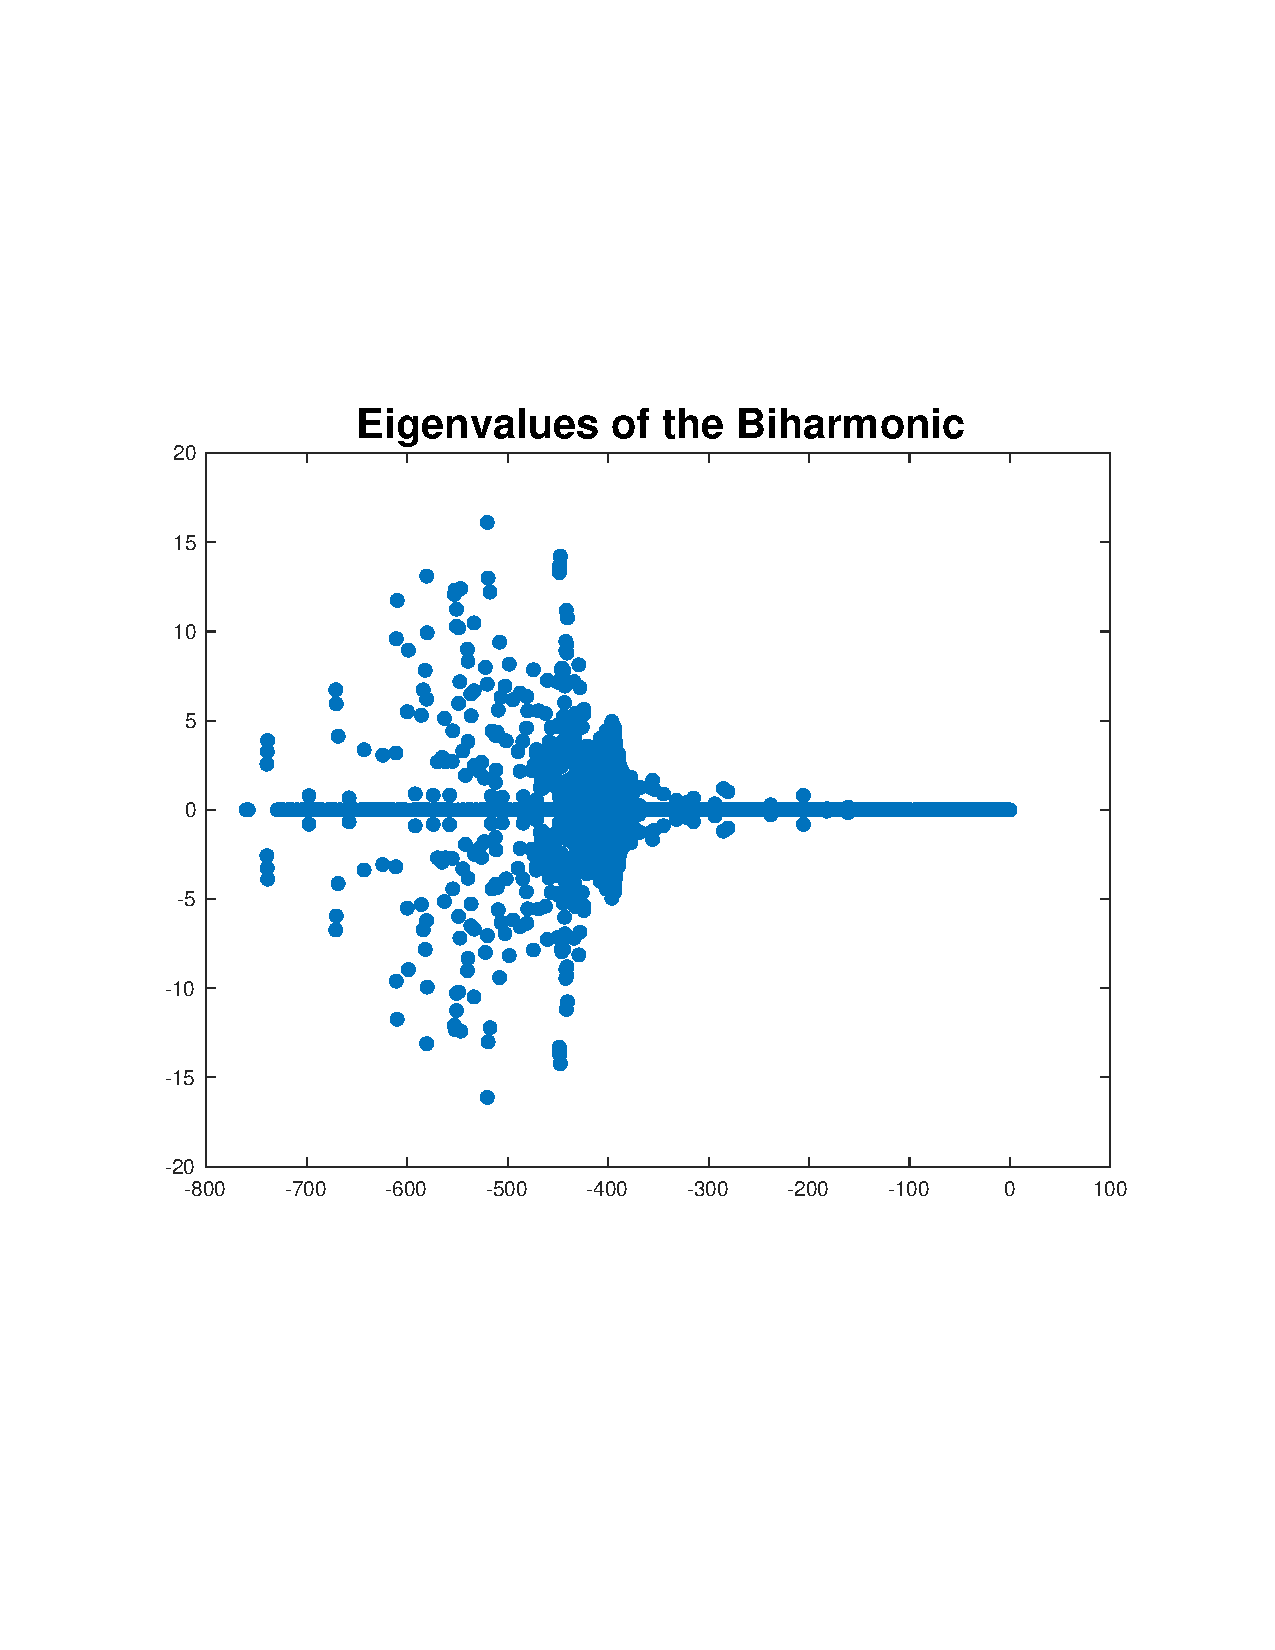
\includegraphics[scale = 0.35, trim = {2cm 7cm 2cm 6.5cm}, clip]{../Pictures_Movies/Spectra_Biharm_Torus_40.pdf}
\includegraphics[scale = 0.35, trim = {2cm 7cm 2cm 6.5cm}, clip]{../Pictures_Movies/Spectra_Biharm_Torus_40_streg.pdf}
%\caption{\displaymath{ \Delta t = \frac{\Delta x^4}{36} }}
\end{figure}

\vspace{-10mm}
 
\begin{gather*}
\Delta t = \frac{\Delta x^4}{36}
\end{gather*}
 
\end{frame} 
 
 
%\begin{frame}
%\frametitle{Convergence on the Sphere}
% 
%\end{frame}  


\begin{frame}
\frametitle{Swift-Hohenberg Equation}
 
Finally, the equation:

\begin{gather*}
u_t = -\triangle^2 u - \triangle u + (P-1)u + su^2 - u^3
\end{gather*} 
 
This equation was derived by Swift and Hohenberg in 1977 to study thermal fluctuations on a fluid near the Rayleigh-Benard
convective instability. The function $u$ is the temperature field in a plane horizontal layer of fluid heated from below. 
The parameter $P$ measures how far the temperature is above the minimum temperature required for convection: for $P<0$,
the heating is too small to cause convection, while for $P>0$, convection occurs. The Swift-Hohenberg equation is an example of 
a PDE that exhibits pattern formation, including stripes, spots and spirals.
 
\end{frame}
 
 
 
\begin{frame}
\frametitle{Discretization}
 
The equation can be written as a sum of linear and non-linear terms: 
 
\begin{gather*}
u_t = \underbrace{-\triangle^2 u - \triangle u + (P-1)u}_{=:Lu} + \underbrace{su^2 - u^3}_{=:Nu}
\end{gather*} 
 
\begin{itemize}
\item Linear part is very stiff (large eigenvalues), but can be inverted - treat implicitly.
\item Nonlinear part is very difficult to invert - treat explicitly.  
\end{itemize} 
 
\end{frame} 



\begin{frame}
\frametitle{Time Stepping}
 
Possible implicit-explicit time stepping schemes: \vspace{5mm}
 
\begin{itemize}
\item IMEX Euler:
\begin{gather*}
\left( I - \Delta t L \right) u^{n+1} = u^n + \Delta t N u^n
\end{gather*}
\item Semi-implicit Backward Differentiation Formula (SBDF2)
\begin{gather*}
\left( 3I - 2\Delta t L \right) u^{n+1} = 4u^n + 4\Delta t Nu^n - u^{n-1} - 2\Delta t Nu^{n-1} 
\end{gather*}   
\item Many more ...
\end{itemize} 
 
\end{frame} 



\begin{frame} 
 
\begin{center}
\Huge{Let's watch some videos.}
\end{center} 
 
\end{frame} 

 
 
\begin{frame} 
 
\begin{center}
\Huge{Thank you for your attention!}
\end{center} 
 
\end{frame} 
 
 
 
%\begin{frame}
%\frametitle{Videos} 
% 
% 
%\movie[width=11cm,height=8cm, poster]{}{../Pictures_Movies/SH_Torus100_2.avi}
% 
% 
%\end{frame}  
 
 
 
 
 
%\begin{frame}
%\frametitle{References}
% 
% 
%\begin{thebibliography}{9}
%\bibitem{implcpm} 
%The Implicit Closest Point Method for the Numerical Solution of Partial Differential Equations on Surfaces.
%\textit{SIAM J. SCI. COMPUT. 2009 Society for Industrial and Applied Mathematics Vol. 31, No. 6, pp. 4330-4350}
% 
%\bibitem{implcpm} 
%The Implicit Closest Point Method for the Numerical Solution of Partial Differential Equations on Surfaces.
%\textit{SIAM J. SCI. COMPUT. 2009 Society for Industrial and Applied Mathematics Vol. 31, No. 6, pp. 4330-4350} 
% 
%
%\end{thebibliography} 
%  
%\end{frame} 
 
 
 
 
 
 
\end{document} 
 
 
 
 
 
 
 
 
 
 
 
 
 
 
  
 
 
 